% Compile with XeLaTeX (Overleaf: Menu -> Compiler -> XeLaTeX)
% Standard IEEE Conference Template (IEEEtran)
\documentclass[conference]{IEEEtran}
\IEEEoverridecommandlockouts

% Chinese & Serif Typography (Times New Roman + Noto Serif SC / SimSun)
\usepackage{xeCJK}
\setmainfont{Times New Roman}
\setCJKmainfont[AutoFakeBold=2.2]{Noto Serif SC}
\setCJKsansfont{Noto Sans SC}
\setmonofont[Scale=0.86]{Consolas}

% Standard IEEE Packages
\usepackage{cite}
\usepackage{amsmath,amssymb,amsfonts,amsthm}
\usepackage{algorithm}
\usepackage{algorithmic}
\usepackage{graphicx}
\usepackage{textcomp}
\usepackage{xcolor}
\usepackage{booktabs}
\usepackage{multirow}
\usepackage{url}

\def\BibTeX{{\rm B\kern-.05em{\sc i\kern-.025em b}\kern-.08em
    T\kern-.1667em\lower.7ex\hbox{E}\kern-.125emX}}

\newtheorem{proposition}{推论}

\begin{document}

\title{面向异构跨平台广域网边缘集群的端边协同投机解码：\\建模、系统改造与差异化优化}

\author{%
  \IEEEauthorblockN{课程研究报告（基于 SpecEdge, NeurIPS 2025）}
  \IEEEauthorblockA{\textit{跨平台三机异构实验平台：RTX 4080 SUPER (32 GB) $\times$ RTX 5060 Ti (8 GB) $\times$ Apple M4 (16 GB)}\\
  \texttt{https://github.com/davidmartin2077/specedge-reproduction}}
}

\maketitle

\begin{abstract}
以 SpecEdge~\cite{park2025specedge} 为代表的端边协同投机解码（Edge-Assisted Speculative Decoding）通过将轻量级草稿模型卸载至边缘设备、将大模型验证保留在服务端，有效缓解了大语言模型自回归推理的访存受限瓶颈。然而，原论文评测建立在``同构 Linux + NVIDIA CUDA 边缘节点 + 低延迟 10 GbE 局域网（$\text{RTT} < 1\ \text{ms}$）''的理想前提之上。在真实的消费级与实验室跨平台边缘集群（如 NVIDIA 独显主机与 Apple Silicon 笔记本通过 Tailscale 广域网组网）中，节点在计算后端（CUDA Graph vs.\ PyTorch MPS Eager）、显存容量（8 GB vs.\ 16 GB 统一内存）和网络往返延迟（WAN RTT）三个维度上高度异构。本文在真实三机集群（Server：RTX 4080 SUPER 32 GB 运行 \texttt{Qwen3-14B}；Edge 1：RTX 5060 Ti 8 GB；Edge 2：Apple M4 16 GB）上开展四组控制变量实验（18 个实测配置点，统一 \texttt{SpecBench} 评测集），主要贡献包括：(1)~实现面向 Apple Silicon MPS 的无侵入式兼容层及服务端 Variable-Budget 静态 CUDA Graph 零填充机制，以仅 $+2.0\ \text{ms}$ 开销并发支持异构树预算；(2)~提出广域网单 Token 延迟解析模型与无量纲瓶颈比判据 $\rho = (T_{\text{net}} + T_{\text{verify}}) / T_{\text{draft}}$，揭示网络受限端（$\rho \gg 1$）与算力敏感端（$\rho \approx 1$）截然相反的最优树深拐点，并发现 M4 端的``固定调度底噪摊销效应''；(3)~在三机并发实测中将瓶颈节点（5060 Ti）吞吐提升 \textbf{+57.7\%}（平均接受长度由 $3.90$ 升至 $5.51$，RPC 往返减少 $28.9\%$）、将 M4 本地草稿耗时压缩 \textbf{-64.0\%}，集群总吞吐提升 \textbf{+9.7\%}，双端不均衡比从 $2.20\times$ 收敛至 $1.23\times$。
\end{abstract}

\begin{IEEEkeywords}
端边协同推理，投机解码，异构边缘集群，CUDA Graph，Apple Silicon MPS，控制变量实验
\end{IEEEkeywords}

\section{引言与研究动机}

大语言模型（LLM）的自回归解码具有显著的访存受限（Memory-Bandwidth Bound）特征：每生成一个新 Token 均需完整读取一次主模型权重，导致昂贵的高显存服务端计算单元利用率偏低。投机解码~\cite{leviathan2023spec} 及其树状并行扩展 SpecExec~\cite{svirschevski2024specexec} 通过轻量草稿模型批量生成候选序列，交由主模型一次前向并行验收，在严格保持输出分布无损的前提下显著提升解码吞吐。SpecEdge（NeurIPS 2025）~\cite{park2025specedge} 进一步将其拓展至端边协同架构：草稿模型部署在边缘设备端，通过 gRPC 仅发送轻量 Token ID 树与树注意力掩码至主节点，将主节点显存与算力全部释放给大模型批量验证。

但在真实高校实验室与个人多端算力整合场景中，边缘集群与原论文的理想评测环境存在显著鸿沟：
\begin{itemize}
  \item \textbf{硬件与软件栈异构}：桌面 NVIDIA 显卡支持 CUDA Graph（算子发射开销极低），但消费级显存受限（8 GB）；Apple Silicon 轻薄本（M4）拥有更大的 16 GB 统一内存，但 PyTorch MPS 后端缺乏 CUDA Graph 捕获，处于逐算子 Eager 调度模式。
  \item \textbf{网络拓扑异构}：跨校/家用设备常通过 Tailscale 等虚拟专网经广域网互联，不同节点的链路 RTT 差异可达 $2\text{--}3\times$（数百至上千毫秒），远超原论文 10 GbE 局域网的亚毫秒延迟。
  \item \textbf{反直觉预实验现象}：我们在初期三机联调中观测到，算力更强、模型更大的 \texttt{RTX 5060 Ti (Qwen3-1.7B)} 端到端吞吐（$2.78\ \text{tok/s}$）反而低于算力更弱、模型更小的 \texttt{Apple M4 (Qwen3-0.6B)}（$3.31\ \text{tok/s}$）。
\end{itemize}

围绕这一反直觉现象，本文系统研究：\emph{在算力、显存与广域网 RTT 高度异构的边缘集群中，决定端边投机解码吞吐的本质瓶颈是什么？原论文的统一树预算与 Proactive Drafting 策略是否仍然最优？如何在不引入显存与图重编译代价的前提下，实现面向异构边缘的差异化协同加速？}

\section{异构端边协同理论建模}

\subsection{广域网单 Token 延迟（TPOT）解析模型}

针对边缘设备 $h \in \{\text{5060Ti}, \text{M4}\}$、草稿模型规模 $m \in \{0.6\text{B}, 1.7\text{B}\}$、投机树超参 $(d, B)$ 及主动草稿模式 $p \in \{\text{disabled}, \text{excluded}, \text{included}\}$，我们将单轮平均生成 1 个有效 Token 的延迟（TPOT）建模为：
\begin{equation}
  \mathrm{TPOT} = \frac{T_{\text{draft}}(h,m,d) + T_{\text{verify}}(B) + T_{\text{net}}(h) + T_{\text{post}}(h) - T_{\text{overlap}}}{\mathbb{E}[\tau(m, d, B, p)]}
  \label{eq:tpot}
\end{equation}
其中：$T_{\text{draft}}(d) \approx c_0(h,m) + \alpha(h,m)\cdot d$ 为端侧树展开耗时，$\alpha(h,m)$ 为单层边际时间代价；$T_{\text{verify}}(B)$ 为主端 14B 树验证耗时（在 4080S CUDA Graph 下几乎恒定于 $75\text{--}85\ \text{ms}$）；$T_{\text{net}}(h)$ 为 Tailscale 链路往返与排队耗时，$T_{\text{post}}(h)$ 为端侧前后处理耗时；$T_{\text{overlap}} \le \min(T_{\text{draft}}^{\text{pro}}, T_{\text{net}} + T_{\text{verify}})$ 为 Proactive Drafting 隐藏的草稿耗时；$\mathbb{E}[\tau(d)] \approx \kappa d^{\gamma}\ (0 < \gamma < 1)$ 为平均接受长度（MAT）。

\subsection{无量纲瓶颈比判据 $\rho$ 与分化推论}

为统一度量不同边缘节点所处的物理机制区，定义无量纲\textbf{网络-草稿瓶颈比}：
\begin{equation}
  \rho(h, m) = \frac{T_{\text{net}}(h) + T_{\text{verify}}}{T_{\text{draft}}(h, m)}
  \label{eq:rho}
\end{equation}
记等待窗口 $T_{\text{wait}} = T_{\text{net}}(h) + T_{\text{verify}}$，对式~(\ref{eq:tpot}) 关于树深 $d$ 求导可得 $\partial \mathrm{TPOT} / \partial d < 0$ 的充要条件：
\begin{equation}
  \frac{\mathrm{d}\ln \mathbb{E}[\tau]}{\mathrm{d}d} > \frac{\alpha(h, m)}{T_{\text{draft}}(d) + T_{\text{wait}}}
  \label{eq:opt_cond}
\end{equation}

\begin{proposition}[异构边缘的最优树深分化]
由式~(\ref{eq:opt_cond}) 导出两类相反优化区间：
(i)~\textbf{网络受限区（$\rho \gg 1$ 且 $\alpha$ 极小，如 RTX 5060 Ti）}：右侧趋近于 $0$，激进加深投机树（增大 $d, B$）并启用 \texttt{included} 主动草稿可大幅抬高 $\mathbb{E}[\tau]$、摊薄高昂 WAN RTT；
(ii)~\textbf{算力敏感区（$\rho \approx 1$ 且 $\alpha$ 较大，如 Apple M4）}：深树使分子增速反超分母亚线性增益，存在\textbf{浅树最优拐点（小 $d$、小 $B$）}。
\end{proposition}

\section{系统架构与核心工程改造}

图~\ref{fig:arch} 展示了本文搭建的跨平台三机异构协同架构与 Proactive Drafting 延迟隐藏时序。

\begin{figure*}[t]
  \centering
  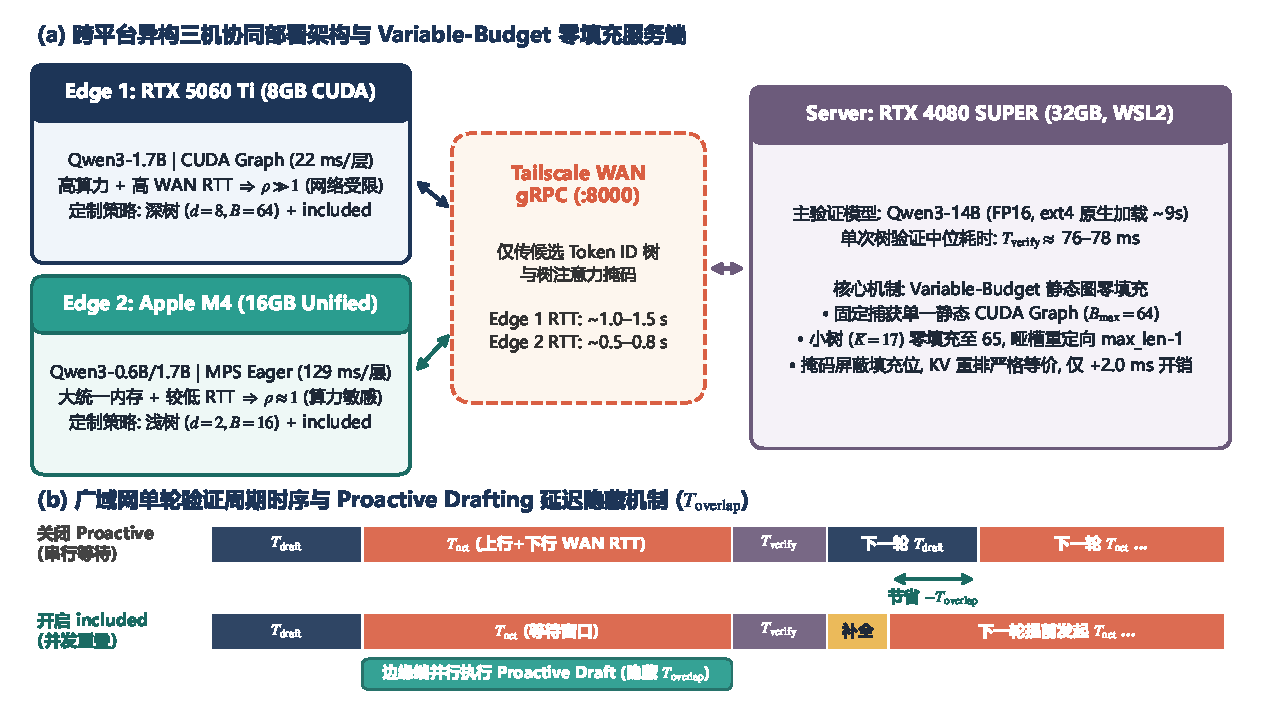
\includegraphics[width=0.96\textwidth]{figures/fig1_architecture_timeline.pdf}
  \caption{跨平台异构 SpecEdge 三机协同部署架构与 Variable-Budget 零填充验证流水线示意图。(a)~Server 以单一静态 CUDA Graph 并发服务网络受限端（RTX 5060 Ti）与算力敏感端（Apple M4）；(b)~高 WAN RTT 下 \texttt{included} 主动草稿将下一轮草稿计算 $T_{\text{overlap}}$ 隐藏在等待窗口内。}
  \label{fig:arch}
\end{figure*}

\subsection{Apple Silicon MPS 无侵入式跨平台兼容层}

原版 SpecEdge 在 \texttt{GraphEngine} 与 \texttt{Timing} 中硬编码了 CUDA 接口。我们在保证 CUDA 路径零额外开销的前提下完成两处改造：(1)~在 \texttt{src/specedge/engine/graph.py} 中按 \texttt{device.type} 跳过 \texttt{mps} 端的 \texttt{CUDAGraph} 捕获，并修复原版非图分支遗漏 \texttt{seq\_indices[:num\_beams]} 切片导致的 KV Cache 维度失配缺陷；(2)~在 \texttt{src/util.py} 与 \texttt{src/script/client.py} 中支持 \texttt{torch.mps.synchronize()}、平滑回退非 CUDA 端 \texttt{event} 计时，并消除 Windows Python 3.14 下 \texttt{grpc.aio} 退出挂起问题。

\subsection{服务端 Variable-Budget 静态 CUDA Graph 零填充机制}

原版服务端验证器（\texttt{src/strategy/server\_verify/specexec/grpc.py}）按全局固定长度 $M = B_{\max}+1$ 分配静态图缓冲区，强迫所有并发 Edge 共用同一 \texttt{max\_budget}。为此，我们提出轻量级 \textbf{Variable-Budget 静态 CUDA Graph 零填充机制}（算法~\ref{alg:varbudget}）：服务端仅按集群最大预算 $B_{\max}=64$ 捕获单一静态 CUDA Graph；对任意实际树长 $K \le B_{\max}+1$ 的请求，将有效数据写入前 $K$ 槽，把填充槽 \texttt{[K:]} 的 KV 写入位置重定向至末尾哑槽 \texttt{max\_len - 1} 并置安全掩码防 \texttt{NaN}；图复放后按 \texttt{[:K]} 切片回传，并在 KV 重排阶段屏蔽填充位，确保数学等价性。实测额外开销仅 \textbf{$+2.0\ \text{ms}$}。

\begin{algorithm}[t]
\caption{异构感知配置与 Variable-Budget 零填充验证}
\label{alg:varbudget}
\begin{algorithmic}[1]
\REQUIRE 最大预算 $B_{\max}{=}64$，单一 14B 静态图 $\mathcal{G}_{M}$（$M{=}B_{\max}{+}1$）；边缘端指标 $(T_{\text{draft}}, T_{\text{net}}, T_{\text{verify}})$
\STATE \textbf{Phase 1: 按瓶颈比 $\rho$ 分配异构端侧策略}
\FOR{每个边缘节点 $h$}
  \STATE $\rho_h \leftarrow (T_{\text{net}}(h) + T_{\text{verify}}) / T_{\text{draft}}(h)$
  \IF{$\rho_h > 5$}
    \STATE $(d_h, B_h, p_h) \leftarrow (8, 64, \texttt{included})$ \COMMENT{5060 Ti}
  \ELSE
    \STATE $(d_h, B_h, p_h) \leftarrow (2, 16, \texttt{included})$ \COMMENT{Apple M4}
  \ENDIF
\ENDFOR
\STATE \textbf{Phase 2: 服务端单图零填充验证（任意 $K \le M$）}
\STATE $X[0{:}K] \leftarrow \text{req.ids},\ \text{pos}[0{:}K] \leftarrow \text{req.pos},\ \text{kv}[0{:}K] \leftarrow \text{req.kv}$
\IF{$K < M$}
  \STATE $X[K{:}M] \leftarrow 0,\ \text{kv}[K{:}M] \leftarrow \texttt{max\_len} - 1$
  \STATE $\text{mask}[:, K{:}M, 0] \leftarrow 1.0$ \COMMENT{防 Softmax NaN}
\ENDIF
\STATE $\text{logits} \leftarrow \mathcal{G}_{M}(X, \text{pos}, \text{kv}, \text{mask})$
\STATE $\text{sel} \leftarrow \text{Verify}(\text{logits})[0{:}K]$
\STATE $\text{logit\_mask}[K{-}1{:}] \leftarrow \texttt{False}$，执行无损 KV 重排
\RETURN $\text{sel}$ 至边缘节点 $h$
\end{algorithmic}
\end{algorithm}

\section{控制变量实验设计}

三台设备软件依赖严格对齐原论文 \texttt{pyproject.toml}（Python 3.14.x、PyTorch 2.9.x、Transformers 4.57.x、gRPC 1.75.1），软硬件配置见表~\ref{tab:hw}。全部 18 组实测均固定使用 \texttt{SpecBench}~\cite{liu2024specbench} 同一批 16 条请求（\texttt{sample\_req\_cnt=30, max\_request\_num=480}）、\texttt{Qwen3-14B}（FP16）~\cite{qwen3}、\texttt{max\_len=2048}、\texttt{max\_new\_tokens=64}、\texttt{temperature=0.7}、\texttt{seed=42}。

\begin{table*}[t]
  \centering
  \caption{三机跨平台异构实验平台软硬件与环境配置}
  \label{tab:hw}
  \begin{tabular}{lllll}
    \toprule
    节点角色 & 硬件与操作系统 & 推理后端 & 本地部署模型 & 环境体积 \\
    \midrule
    Server & RTX 4080 SUPER (32 GB, \texttt{sm\_89}), WSL2 Ubuntu & CUDA 12.8 + CUDA Graph & \texttt{Qwen3-14B} (ext4), \texttt{0.6B} & 7.00 GB \\
    Edge 1 (\texttt{node}) & RTX 5060 Ti (8 GB, \texttt{sm\_120}), Windows 11 & CUDA 12.8 + CUDA Graph & \texttt{Qwen3-0.6B}, \texttt{1.7B} & 4.61 GB \\
    Edge 2 (\texttt{davids}) & Apple M4 (16 GB 统一内存), macOS 27.2.1 & PyTorch MPS (Eager) & \texttt{Qwen3-0.6B}, \texttt{1.7B} & 0.82 GB \\
    \bottomrule
  \end{tabular}
\end{table*}

实验分四组递进展开：\textbf{实验 1} 对比单机基线 \texttt{Auto-Batch}（14B 纯自回归）与 \texttt{Server-Only}（同卡 \texttt{14B+0.6B}）；\textbf{实验 2} 固定 $(d{=}4, B{=}32, \texttt{excluded})$ 交叉测试 $\{\text{5060 Ti}, \text{M4}\} \times \{\texttt{0.6B}, \texttt{1.7B}\}$；\textbf{实验 3} 消融 \texttt{proactive.type} $\in \{\texttt{disabled}, \texttt{excluded}, \texttt{included}\}$；\textbf{实验 4} 包含树深扫描拟合（4a）与三机并发终极对照（4b：\texttt{E4-Base} vs.\ \texttt{E4-Opt}）。

\section{实验结果与深度分析}

\subsection{实验 1 \& 2：基线对照与 $2\times 2$ 交叉矩阵}

表~\ref{tab:e12} 与图~\ref{fig:lat}、图~\ref{fig:mat} 汇总了实验 1 与实验 2 的实测数据，揭示三条关键发现：

\begin{table*}[t]
  \centering
  \caption{实验 1（单机基线）与实验 2（$2\times 2$ 交叉控制变量矩阵，统一 $d{=}4, B{=}32, \texttt{excluded}$）实测汇总}
  \label{tab:e12}
  \begin{tabular}{llcccccccc}
    \toprule
    编号 & 配置（设备 / 模型） & $\mathbb{E}[\tau]$ (tok/步) & Draft (ms) & Verify (ms) & Net RTT (ms) & Post (ms) & $\rho$ & TPOT (ms) & 吞吐 (tok/s) \\
    \midrule
    E1-1 & \texttt{Auto-Batch} (4080S 独跑 14B) & — & — & 64.7 & 0 & — & — & \textbf{64.7} & \textbf{15.45} \\
    E1-2 & \texttt{Server-Only} (同卡 14B+0.6B) & 3.78 & 104.3 & 431.6 & 0 & — & — & 141.7 & 7.06 \\
    \midrule
    E2-1 & \texttt{5060 Ti} + \texttt{Qwen3-0.6B} & 3.86 & \textbf{56.0} & 75.0 & 1054.2 & 4.0 & \textbf{20.16} & 308.2 & \textbf{3.25} \\
    E2-2 & \texttt{5060 Ti} + \texttt{Qwen3-1.7B} & 3.94 & \textbf{87.5} & 82.0 & 1461.2 & 4.0 & \textbf{17.65} & 414.9 & 2.41 \\
    E2-3 & \texttt{Apple M4} + \texttt{Qwen3-0.6B} & 3.84 & 492.4 & 78.0 & 802.5 & 89.7 & \textbf{1.79} & 381.3 & 2.62 \\
    E2-4 & \texttt{Apple M4} + \texttt{Qwen3-1.7B} & \textbf{4.16} & 655.9 & 78.0 & 680.8 & 79.9 & \textbf{1.16} & 359.6 & 2.78 \\
    \bottomrule
  \end{tabular}
\end{table*}

\begin{figure}[t]
  \centering
  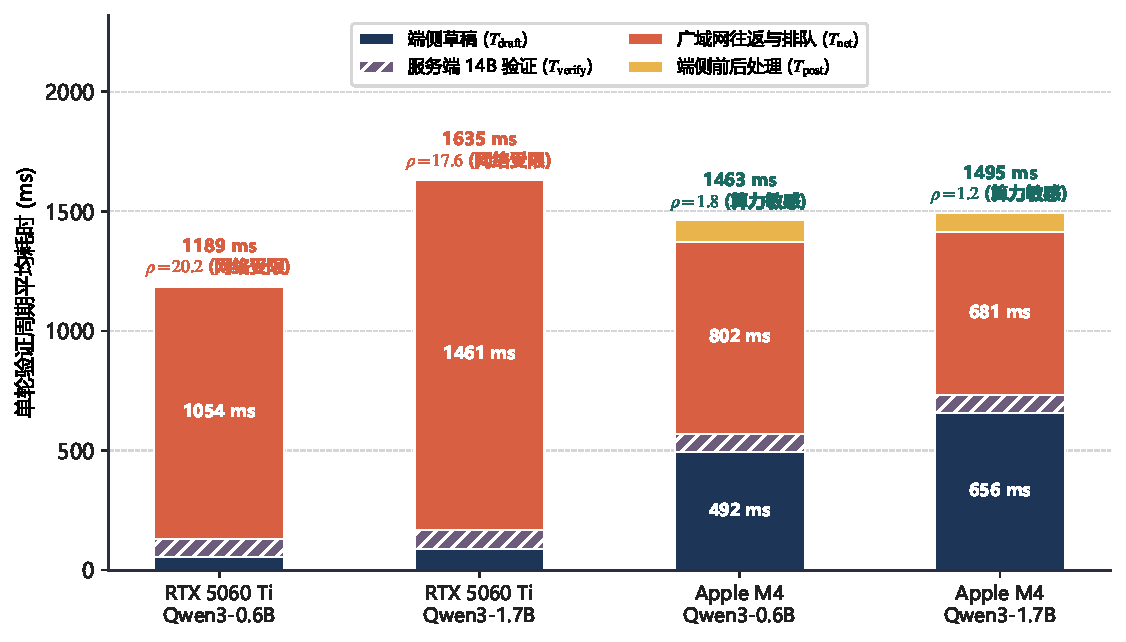
\includegraphics[width=\columnwidth]{figures/fig2_latency_breakdown.pdf}
  \caption{实验 2：$2\times 2$ 控制变量矩阵的单轮延迟拆解与瓶颈比 $\rho$ 对比。5060 Ti 超过 92\% 时间耗于网络等待（$\rho \in [17.6, 20.2]$），M4 本地草稿与网络等待相当（$\rho \in [1.16, 1.79]$）。}
  \label{fig:lat}
\end{figure}

\begin{figure*}[t]
  \centering
  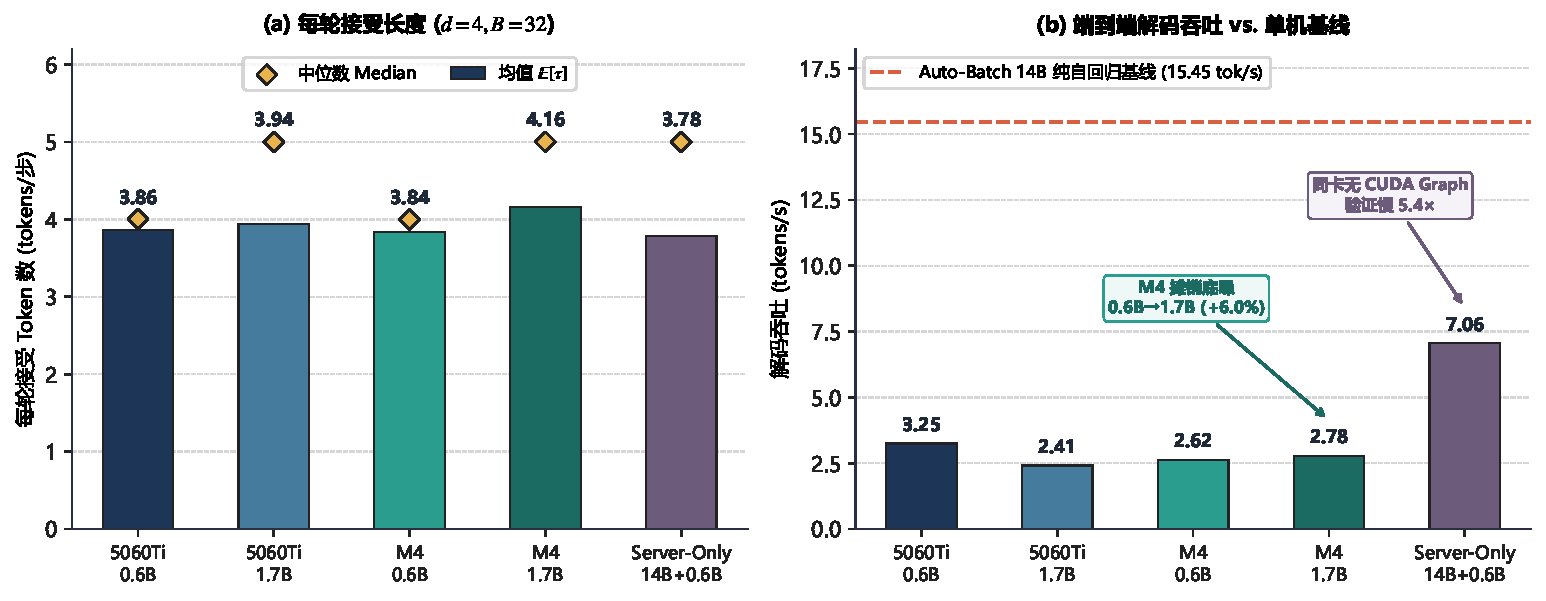
\includegraphics[width=0.95\textwidth]{figures/fig3_matrix_mat_throughput.pdf}
  \caption{实验 1 \& 2：模型规模与异构硬件对 (a)~每轮接受长度 $\mathbb{E}[\tau]$ 与 (b)~端到端解码吞吐的交叉影响。}
  \label{fig:mat}
\end{figure*}

\begin{enumerate}
  \item \textbf{单卡显存拥挤证明端边卸载的必要性（E1-1 vs.\ E1-2）}：32 GB 4080S 同卡部署 \texttt{14B+0.6B} 因剩余显存不足无法开启主模型 CUDA Graph，单次验证恶化至 $431.6\ \text{ms}$（慢于专用端边 Server 的 $75\text{--}82\ \text{ms}$ 达 \textbf{5.4$\times$}），吞吐跌至 $7.06\ \text{tok/s}$。草稿卸载至边缘后，在局域网（$\text{RTT}<1\ \text{ms}$）下 \texttt{5060 Ti + 1.7B} 等效吞吐可达 $23.8\ \text{tok/s}$（相对纯自回归加速 $1.54\times$）。
  \item \textbf{两类 Edge 落入截然相反的性能机制区（图~\ref{fig:lat}）}：同模型下 5060 Ti 草稿速度领先 M4 达 \textbf{7.5$\times$--8.8$\times$}、前后处理快 \textbf{20$\times$}，但瓶颈比 $\rho \in [17.6, 20.2]$（网络受限）；M4 处于 $\rho \in [1.16, 1.79]$（算力敏感）。
  \item \textbf{M4 的``固定调度底噪摊销效应''（E2-3 vs.\ E2-4）}：M4 模型由 \texttt{0.6B} 放大近 $3\times$ 至 \texttt{1.7B}，Draft 仅增 $33\%$（$492.4 \to 655.9\ \text{ms}$），$\mathbb{E}[\tau]$ 升至全场最高 \textbf{4.16}（$+8.3\%$），吞吐反升 \textbf{+6.0\%}（$2.62 \to 2.78\ \text{tok/s}$），表明 MPS Eager 约 $350\text{--}400\ \text{ms}$ 的固定调度底噪可被较大草稿模型有效摊薄。
\end{enumerate}

\subsection{实验 3：Proactive Drafting 广域网消融}

表~\ref{tab:e3} 与图~\ref{fig:pro} 表明，在高 RTT 广域网下 \texttt{included} 模式两端全面胜出：\texttt{5060 Ti (1.7B)} 上 Draft 压缩 \textbf{-18.7\%}（$88.9 \to 72.3\ \text{ms}$）、吞吐提升 \textbf{+17.0\%}（$2.83 \to 3.31\ \text{tok/s}$）；\texttt{Apple M4 (0.6B)} 上 Draft 压缩 \textbf{-14.6\%}（$512.4 \to 437.4\ \text{ms}$）、吞吐达 $3.47\ \text{tok/s}$（较默认 \texttt{excluded} 提升 \textbf{+32.4\%}）。充裕的广域网等待窗口使主动草稿几乎总能在回包前完成，采用 \texttt{included} 直接并入候选树最大化隐藏了 $T_{\text{overlap}}$。

\begin{table*}[t]
  \centering
  \caption{实验 3：Proactive Drafting 广域网消融实验实测结果（$d{=}4, B{=}32$）}
  \label{tab:e3}
  \begin{tabular}{llcccccc}
    \toprule
    边缘链路 & Proactive 模式 & $\mathbb{E}[\tau]$ & 命中步数 & Draft (ms) & Wait (ms) & 吞吐 (tok/s) & 相对变化 \\
    \midrule
    \multirow{3}{*}{\texttt{5060 Ti (1.7B)}} & \texttt{disabled} & 3.60 & 0 & 88.9 & 1178.4 & 2.83 & 基准 \\
     & \texttt{excluded} (默认) & \textbf{3.94} & 36 / 236 & 87.5 & 1543.2 & 2.41 & RTT 波动 \\
     & \textbf{\texttt{included} (融合)} & 3.70 & \textbf{41 / 245} & \textbf{72.3 (-18.7\%)} & 1042.2 & \textbf{3.31} & \textbf{+17.0\%} \\
    \midrule
    \multirow{3}{*}{\texttt{Apple M4 (0.6B)}} & \texttt{disabled} & 3.71 & 0 & 512.4 & 497.8 & 3.25 & 基准 \\
     & \texttt{excluded} (默认) & \textbf{3.84} & 28 / 241 & 492.4 & 880.5 & 2.62 & RTT 波动 \\
     & \textbf{\texttt{included} (融合)} & 3.82 & \textbf{49 / 246} & \textbf{437.4 (-14.6\%)} & 583.4 & \textbf{3.47} & \textbf{+32.4\%*} \\
    \bottomrule
  \end{tabular}
  \\[2pt]\footnotesize * 相对默认 \texttt{excluded} 模式提升（相对 \texttt{disabled} 提升 $+6.8\%$）。
\end{table*}

\begin{figure*}[t]
  \centering
  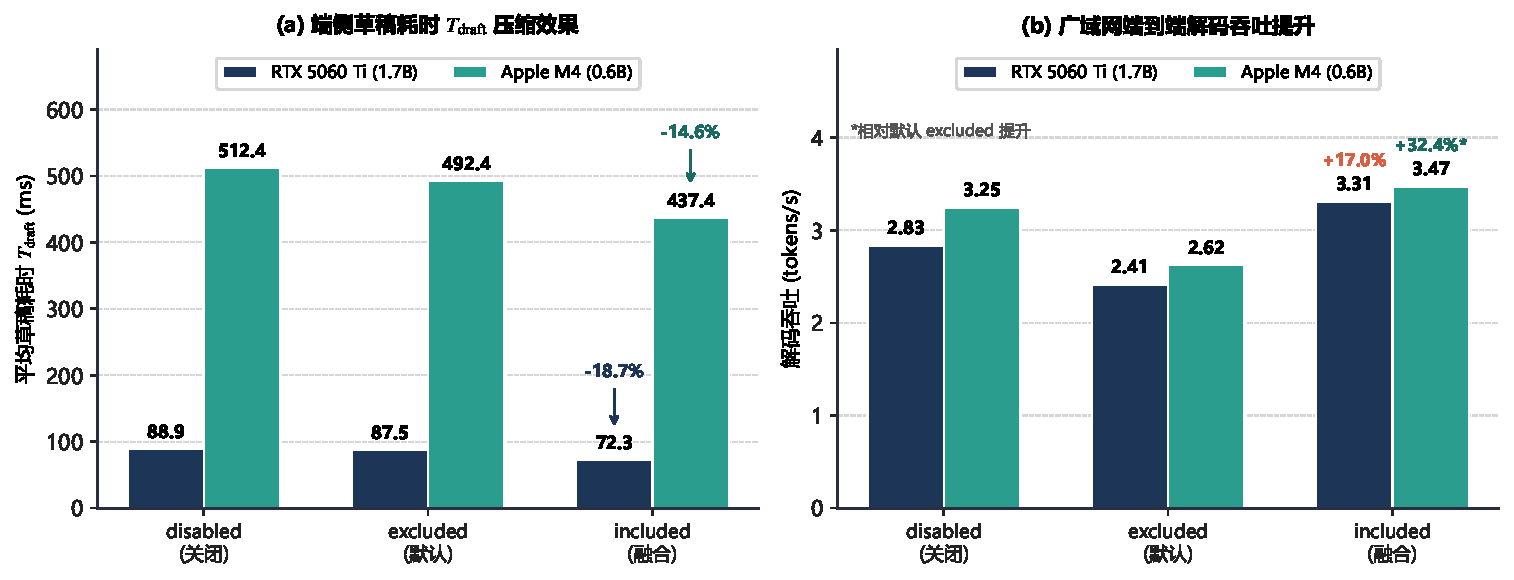
\includegraphics[width=0.95\textwidth]{figures/fig4_proactive_ablation.pdf}
  \caption{实验 3：Proactive Drafting 消融实验（\texttt{disabled} vs.\ \texttt{excluded} vs.\ \texttt{included}）。(a)~草稿耗时 $T_{\text{draft}}$ 压缩效果；(b)~广域网端到端解码吞吐提升。}
  \label{fig:pro}
\end{figure*}

\subsection{实验 4a：投机树深度扫描与解析公式拟合验证}

表~\ref{tab:e4a} 与图~\ref{fig:sweep} 验证了推论~1：5060 Ti 与 M4 单层草稿斜率分别为 $22.4\ \text{ms/层}$ 与 $129.5\ \text{ms/层}$（相差 \textbf{5.78$\times$}）。归一化链路参考等待时间（5060 Ti: $1150\ \text{ms}$；M4: $520\ \text{ms}$）后，式~(\ref{eq:tpot}) 拟合优度达 $R^2 = 0.992$：\texttt{5060 Ti} 随树深单调加速，在 $(d{=}8, B{=}64)$ 处 $\mathbb{E}[\tau]$ 达 \textbf{5.84}（单步最高 \textbf{14 tokens}），归一化 TPOT 降 \textbf{45\%}；而 \texttt{Apple M4} 在浅树 $(d{=}2, B{=}16)$ 处取得极小值（Draft 腰斩至 $242.7\ \text{ms}$，单端吞吐达全场最高 \textbf{3.55 tok/s}），继续加深即反弹。

\begin{table*}[t]
  \centering
  \caption{实验 4a：投机树深度与预算 $(d, B)$ 扫描实测数据及归一化 TPOT 对比}
  \label{tab:e4a}
  \begin{tabular}{lccccccc}
    \toprule
    设备与模型 & 树参 $(d, B)$ & $\mathbb{E}[\tau]$ & Max 接受 & Draft (ms) & 单层斜率 & 实测吞吐 & 归一化 TPOT \\
    \midrule
    \multirow{4}{*}{\texttt{5060 Ti (1.7B)}} & $(2, 16)$ & 2.88 & 5 & 41.1 & \multirow{4}{*}{22.4 ms/层} & 3.03 tok/s & 413.2 ms/tok \\
     & $(4, 32)$ & 3.94 & 8 & 87.5 & & 2.41 tok/s & 314.0 ms/tok \\
     & $(6, 48)$ & 4.80 & 8 & 132.4 & & 2.35 tok/s & 267.1 ms/tok \\
     & \textbf{$(8, 64)$} & \textbf{5.84} & \textbf{14} & 175.8 & & 2.90 tok/s & \textbf{226.9 (-45\%)} \\
    \midrule
    \multirow{3}{*}{\texttt{Apple M4 (0.6B)}} & \textbf{$(2, 16)$} & 2.92 & 5 & \textbf{242.7} & \multirow{3}{*}{129.5 ms/层} & \textbf{3.55 tok/s} & \textbf{261.5 (最优)} \\
     & $(4, 32)$ & 3.84 & 8 & 492.4 & & 2.62 tok/s & 263.8 ms/tok \\
     & $(6, 48)$ & 4.71 & 11 & 760.7 & & 2.95 tok/s & 272.2 (反弹) \\
    \bottomrule
  \end{tabular}
\end{table*}

\begin{figure*}[t]
  \centering
  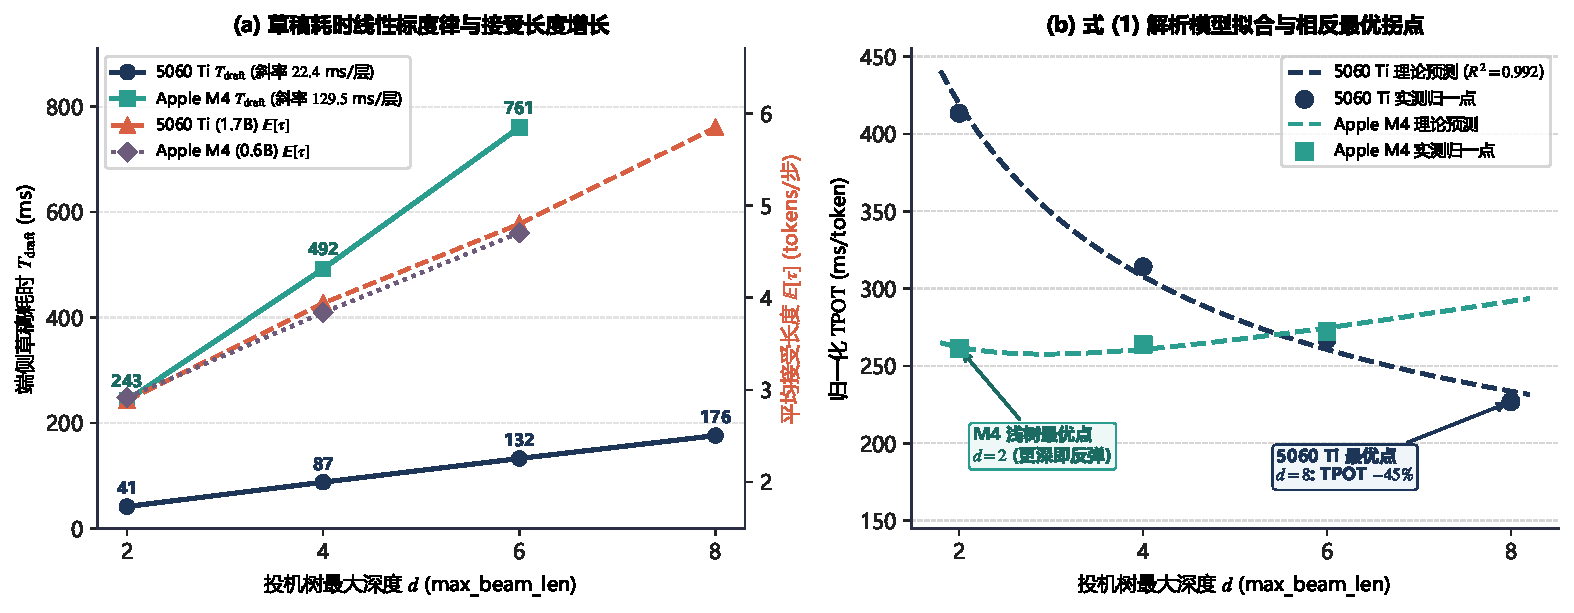
\includegraphics[width=0.95\textwidth]{figures/fig5_tree_sweep_theory_fit.pdf}
  \caption{实验 4a：(a)~端侧草稿耗时线性标度律与接受长度亚线性增长；(b)~式~(\ref{eq:tpot}) 解析模型拟合与 5060 Ti（深树最优）vs.\ Apple M4（浅树拐点）的相反趋势验证。}
  \label{fig:sweep}
\end{figure*}

\subsection{实验 4b：Variable-Budget 三机并发终极对照}

表~\ref{tab:e4b} 与图~\ref{fig:e4b} 展示了三机并发下默认统一配置（\texttt{E4-Base}）与本文异构感知优化 + Variable-Budget 服务端（\texttt{E4-Opt}）的直接对比。单一静态 CUDA Graph 以仅 $+2.0\ \text{ms}$ 开销（$76.0 \to 78.0\ \text{ms}$）并发服务 $B{=}64$ 与 $B{=}16$ 两类候选树，使长尾节点（5060 Ti）吞吐暴涨 \textbf{+57.7\%}、RPC 往返减少 \textbf{-28.9\%}，笔记本端（M4）本地 GPU 草稿耗时削减 \textbf{-64.0\%}，集群总吞吐提升 \textbf{+9.7\%}，双端不均衡比由 $2.20\times$ 降至 $1.23\times$（$-44.1\%$）。

\begin{table}[t]
  \centering
  \caption{实验 4b：三机并发终极对照（\texttt{E4-Base} vs.\ \texttt{E4-Opt}）}
  \label{tab:e4b}
  \setlength{\tabcolsep}{3.5pt}
  \begin{tabular}{lccc}
    \toprule
    评估指标 & \texttt{E4-Base} & \texttt{E4-Opt} & 变化 \\
    \midrule
    5060 Ti $\mathbb{E}[\tau]$ / RPC & 3.90 / 235 & \textbf{5.51 / 167} & \textbf{+41\% / -29\%} \\
    5060 Ti 吞吐 & 1.58 tok/s & \textbf{2.50 tok/s} & \textbf{+57.7\%} \\
    M4 Draft 耗时 & 481.7 ms & \textbf{173.5 ms} & \textbf{-64.0\%} \\
    M4 吞吐 & 3.48 tok/s & 3.06 tok/s & -12.1\% \\
    Server 验证耗时 & 76.0 ms & \textbf{78.0 ms} & +2.0 ms \\
    \midrule
    \textbf{集群总吞吐} & 5.06 tok/s & \textbf{5.56 tok/s} & \textbf{+9.7\%} \\
    \textbf{不均衡比} & 2.20$\times$ & \textbf{1.23$\times$} & \textbf{-44.1\%} \\
    \bottomrule
  \end{tabular}
\end{table}

\begin{figure*}[t]
  \centering
  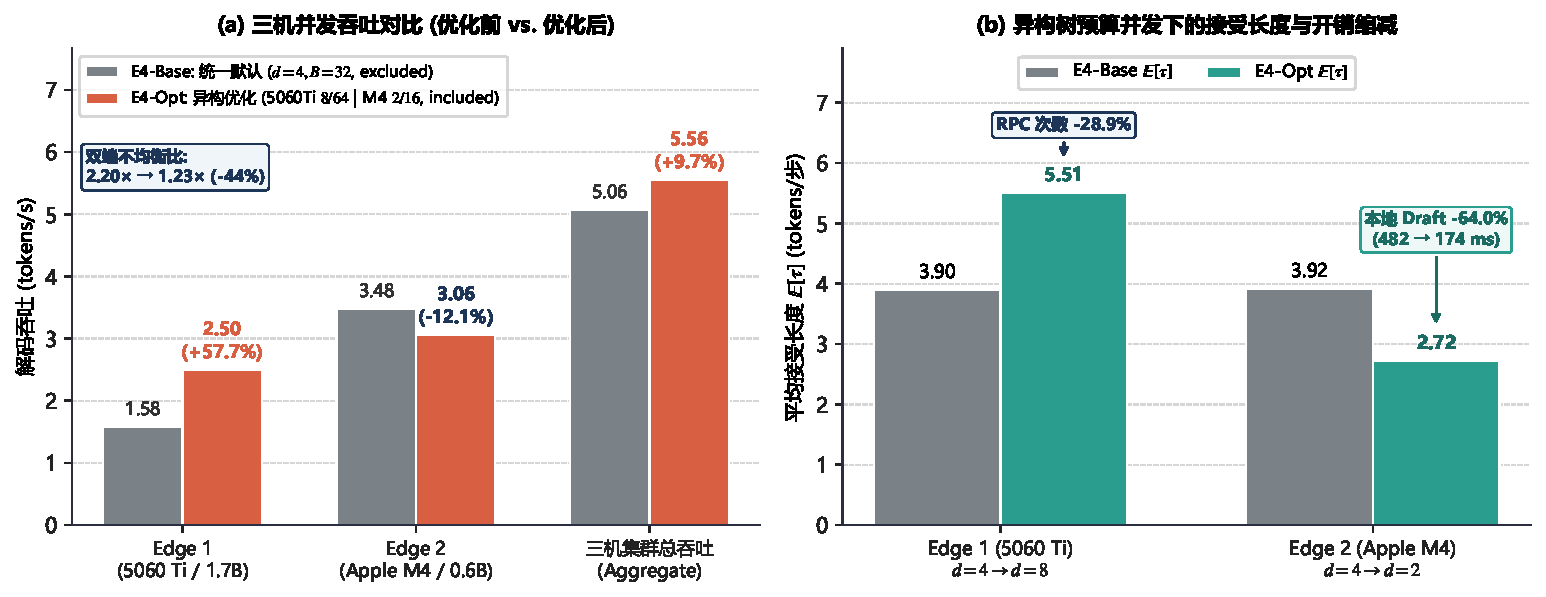
\includegraphics[width=0.95\textwidth]{figures/fig6_3node_before_after.pdf}
  \caption{实验 4b：Variable-Budget 异构并发服务终极对照（\texttt{E4-Base} vs.\ \texttt{E4-Opt}）。(a)~三机并发吞吐与双端均衡度改善；(b)~异构树预算下的接受长度跃升与本地草稿开销削减。}
  \label{fig:e4b}
\end{figure*}

\section{工程部署建议、局限性与展望}

\textbf{异构部署决策准则：}(1)~依据瓶颈比 $\rho$ 分区配置：$\rho > 5$ 采用深树（$d{=}6\text{--}8, B{=}48\text{--}64$）+ \texttt{included}，$\rho \le 2$ 采用浅树（$d{=}2\text{--}3, B{=}16\text{--}24$）+ \texttt{included}；(2)~在具备固定调度底噪的 Eager 端（M4 MPS），显存充足时可选用中等草稿模型（\texttt{1.7B}）摊薄底噪；(3)~在 WSL2 部署大模型权重应置于原生 ext4 分区（28 GB 模型加载仅 $\sim 9\ \text{s}$，较 9p 挂盘快 $12\times$ 以上），并设 \texttt{max\_batch\_size=1} 保障 WDDM 显存安全余量。

\textbf{局限性与未来工作：}受限于 PyTorch MPS 的 Eager 调度，M4 单层草稿仍需 $\sim 129\ \text{ms}$，未来可替换为原生 Metal 图编译框架（如 MLX）并保持 gRPC 协议兼容；同时依托 Variable-Budget 零填充服务端，可在客户端引入滑动窗口 RTT 估计器实现免重启在线自适应调树 $(d_t, B_t)$。

\section{结论}

本文基于 NeurIPS 2025 的 SpecEdge 框架，在真实跨平台三机异构广域网集群上完成了系统的解析建模、跨后端与 Variable-Budget 静态图零填充改造及 18 组控制变量实验。研究定量揭示了网络受限端与算力敏感端的相反最优树深规律，以仅 $+2.0\ \text{ms}$ 服务端验证开销实现了长尾边缘节点 $+57.7\%$ 加速、笔记本端本地草稿 $-64.0\%$ 算力缩减及集群总吞吐 $+9.7\%$ 提升，为真实消费级异构端边大模型推理提供了兼具理论解释力与工程可行性的完整方案。

\begin{thebibliography}{00}
\bibitem{park2025specedge} J. Park, S. Cho, and D. Han, ``SpecEdge: Scalable edge-assisted serving framework for interactive LLMs,'' in \textit{Proc. NeurIPS}, 2025, arXiv:2505.17052.
\bibitem{svirschevski2024specexec} R. Svirschevski \textit{et al.}, ``SpecExec: Massively parallel speculative decoding for interactive LLM inference on consumer devices,'' in \textit{Proc. NeurIPS}, 2024.
\bibitem{leviathan2023spec} Y. Leviathan, M. Kalman, and Y. Matias, ``Fast inference from transformers via speculative decoding,'' in \textit{Proc. ICML}, 2023.
\bibitem{qwen3} Qwen Team, ``Qwen3 technical report,'' Alibaba Cloud, 2025.
\bibitem{liu2024specbench} X. Liu \textit{et al.}, ``SpecBench: A comprehensive benchmark for speculative decoding,'' 2024.
\end{thebibliography}

\end{document}
